In diesem Kapitel werden die Rahmen- und Randbedienungen für das methodische Vorgehen der Evaluation großer Sprachmodelle für die Codegenerierung von webbasiertem Code festgehalten. Dies umfasst die Festlegung der verwendeten LLMs, die geprüfte Programmiersprachen, Framework zur Erstellung und Auswertung der Tests und Systeme für die Bereitstellung und Verarbeitung der Ergebnisse. Die Evaluierung der Modelle erfolgt in deutscher Sprache, was die Prompts und die Tests betrifft. Allein die Methodenbezeichnung ist in englischer Sprache.

\section{Definition der Evaluierungsziele}
%*   Dieser Abschnitt stellt sicher, dass die Evaluation messbar und reproduzierbar ist.

%*   Welche Aspekte der Codegenerierung sollen evaluiert werden? (z.B. Korrektheit des generierten Codes, Performance (Ausführungsgeschwindigkeit), Codequalität (Lesbarkeit, Wartbarkeit), Einhaltung von Coding Standards, Sicherheit, etc.)

Ausgehend von den in Kapitel \ref{sec:goals_of_the_work} aufgestellten Thesen dieser Arbeit, werden hier die Konzepte und Designs für die Evaluation und Optimierung besprochen. Es wird dargelegt wie Untersuchen durchgeführt, um valide Aussagen zu den Thesen treffen zu können. Es wird darauf geachtet das die Ergebnisse nachvollziehbar und überprüft werden können.
Die Evaluation soll zeigen, inwieweit die LLMs korrekte Ergebnisse liefern und für die Webanwendungsentwicklung geeignet sind. Bei der Evaluierung der optimierten Abfragen wird der Fokus zusätzlich auf die Codequalität liegen. Hierbei wird auf die Codingstandards der Programmiersprache geachtet, die Lesbarkeit und die Dokumentation innerhalb des Codes bewertet. Für die Evaluation werden wie beim HumanEval-XL Benchmark Test geschrieben und zusätzlich werden Tool zur Codebewertung eingesetzt. Trotz der Wichtigkeit der Aspekte werden bei den Tests Aspekte zur Performance und Sicherheitsaspekte vernachlässigt. Es geht in erster Linie darum zu evaluieren, ob die Brauchbarkeit und Verständlichkeit gegeben ist und sich somit die erste These beweisen lässt, das LLMs zur Steigerung der Effizienz und Verbesserung der Codequalität beitragen.\vspace{0.2cm}

%* Welche konkreten Metriken werden zur Messung dieser Aspekte verwendet? (z.B. Anzahl der Fehler im generierten Code, Ausführungszeit in Millisekunden, statische Codeanalyse-Metriken, etc.)
Für die Messung zur Wahrscheinlichkeit das ein Modell eine korrekte Antwort liefert, wird die \texttt{pass@k} Methode auf die Antworten der Modelle angewandt. Für jede Probe liefert der HumanEval-XL eigene Tests mit. Dieser Test zusammen mit dem generierten Code sollten einen ausführbaren und testbaren Code ergeben. Daraus kann dann mit der \texttt{pass@k} Methode die repräsentative Zuverlässigkeit des Modells für jedes Problem ermittelt und anschließend für das gesamte Modell berechnen.\vspace{0.2cm}

Die Proben aus dem HumanEval-XL Benchmark beschreiben grundlegende Verständnisfragen für die Modelle und sind mit einer einzelnen Funktion zu beantworten. In der Praxis stellen Entwickler komplexere Aufgaben an die Modelle, welche nicht nur als einzelne Funktion umzusetzen sind. Oft werden mehrere Webtechnologien als Antwort erwartet, beispielsweise für Abfragen zu Webseiten könnten hier Technologien aus den Bereichen HTML, CSS, JavaScript und PHP zusammenspielen, um eine funktionsfähige Webanwendung zu generieren. Aus diesem Grund werden für die Optimierung neben dem HumanEval-XL Benchmark noch eigene komplexere Proben mit Tests erstellt. Das Design dieser Proben soll auf objektorientierter Programmierung beruhen und mehrere Probleme der Webprogrammierung abdecken. Hier soll geprüft werden, ob die dritte These bewiesen werden kann und eine Optimierung für die Webanwendungsentwicklung herbeigeführt werden kann, ohne das Modell grundlegend zu ändern.

%---------------------------------------------------------------------------------------------------


\section{Auswahl der LLMs und deren Konfiguration}\label{subsec:llm_selection}
%*   Dieser Abschnitt legt die experimentelle Basis fest

%*   Welche LLMs werden konkret in den Experimenten verwendet? (Begründung basierend auf den Ergebnissen des Grundlagenkapitels)
Für die Evaluation werden experimentell einige freie und kommerzielle Modelle ausgewählt und miteinander verglichen. Hauptsächlich wurden bei den freien Modellen, jene ausgewählt welche den Fokus auf die Codegenerierung legen und mit diesem Argument beworben werden. Als Referenz soll das kommerzielle Modell \textit{Gemini 1.5} dienen, welches durch stetige Verbesserung und einer großen Nutzerzahl erstellt wurde.\vspace{0.2cm}

Im Folgenden werden die ausgewählten LLMs kurz vorgestellt und warum diese gewählt wurden. Die Reihenfolge stellt an dieser Stelle keine Wertung der LLM oder über deren generierten Inhalte dar.\vspace{0.2cm}

Das \textbf{Qwen2.5-Coder}-Modell zeichnet sich durch seine spezialisierte Architektur für die Codegenerierung aus. Trainiert, um sowohl syntaktisch korrekten als auch funktional hochwertigen Code zu produzieren, integriert es fortschrittliche Mechanismen zum Kontextverständnis und semantisch sinnvolle Ausgabe. Es findet Anwendung in verschiedenen Bereichen der Softwareentwicklung, insbesondere in der Web- und Anwendungsprogrammierung. Die Qwen2.5-Coder Modellbeschreibung ist \cite{qwen-2024} und \cite{hui-2024} entnommen und wird in den Arbeiten vertieft.\vspace{0.2cm}

\textbf{Deepseek-Coder-V2} ist die zweite Generation der Deepseek-Coder-Reihe, von der gleichnamigen KI-Entwicklungsfirma DeepSeek und soll verbesserte Fähigkeiten zur Codegenerierung und -optimierung bieten. Das Modell nutzt fortschrittliche Suchalgorithmen, um präzisere und effizientere Codestücke zu erstellen. Es ist insbesondere für seine hohe Genauigkeit bei der Generierung komplexer Algorithmen und Datenstrukturen bekannt. Die Modellbeschreibung ist unter anderem aus \cite{deepseek-ai-2024} und \cite{cui-2024} entnommen. Des Weiteren wird das Modell in beiden Arbeiten mit verschiedenen Open-Source und Close-Source Modellen verglichen.\vspace{0.2cm} 

Die jüngste Innovation der chinesischen KI-Entwicklungsfirma DeepSeek ist das \textbf{DeepSeek-R1} Modell. Mit seiner offiziellen Vorstellung im Januar 2025 erregte es bedeutende Aufmerksamkeit sowohl im Bereich künstlicher Intelligenz als auch an den Finanzmärkten. Laut Unternehmensaussagen gleichwertig zu closed-source -Systemen wie ChatGPT-4 oder Gemini 2.0, demonstriert das R1-Modell eine erhebliche Leistungskraft. Im Rahmen dieser Untersuchung wurde speziell die Version deepseek-r1 analysiert, die über 32 Milliarden Parameter verfügt.\vspace{0.2cm}

Die Modelle \textbf{Llama 3.1-Claude} und \textbf{Llama 3.1} gehören mit 8 Milliarden Parametern zu den kleineren Modellen von Meta. Beide Modelle basieren auf dem LLama3.1 Modell, das Llama3.1-Claude ist aber mit anderen Systemaufforderungen erstellt wurden. Hierfür wurden die Systemaufforderungen vom Claude Sonnet 3.5 der Firma Anthropic’s verwendet, nachzulesen unter \cite{ollama_page_llama31_claude}. Ein ähnliches Modell ist auf Hugging Face veröffentlicht \cite{huggingface_page_llama31_claude}. Eine Modelcard mit weiteren Informationen zum Modell ist zu finden unter \cite{meta-llama-no-date}.\vspace{0.2cm}

Ein weiteres Modell von der KI-Entwicklungsfirma \textbf{Meta}, wurden speziell zur Codegenerierung entwickelt. Hierbei handelt es sich um das Modell \textit{Codellama}, welches mit unterschiedlicher Parameteranzahl evaluiert wird. CodeLlama basiert auf Metas Llama2 Modell wurde im Januar 2024 veröffentlicht.
% Codellama:13b
Zuerst wird das Modell \textit{Codellama:13b} evaluiert. Mit dieser Anzahl von Parametern gehört das Modell zu den kleineren Modellen. Dies wurde die Gewichte auf zwei Bit quantisiert, somit ist die Größe des Modells auf 7,4 GB reduziert wurden.
% Codellama:70b
Die zweite Modellkonfiguration ist das \textit{Codellama:70b} und wurde durch eine Quantisierung Q2\_K von 39 GB auf 25 GB verkleinert. Laut \cite{meta-2023} unterstützt das Modell unter anderem Programmiersprachen wie PHP, welche für die Erstellung für Webanwendungen relevant sind.\vspace{0.2cm}

\textbf{Mistral} ist ein modernes leistungsfähiges Sprachmodell, welches nicht speziell für die Codegenerierung und -analyse entwickelt wurde. Es verwendet fortschrittliche Transformer-Architekturen und ist für eine Vielzahl von Aufgaben einsetzbar. Darunter fallen beispielsweise natürliche Sprachverarbeitung, Textzusammenfassungen, maschinelle Übersetzung und Textklassifizierung. Dieses Modell ausgewählt, um ein Modell zu evaluieren, welches nicht speziell auf Codegenerierungsaufgaben trainiert wurde. In der Arbeit \cite{eberhardinger-2024} wurde Mistral, mit verschiedenen Modelle zur Spielecodegenerierung verglichen. Während in \cite{quan-2024} eine Evaluation für natürlichsprachlicher Erklärungen, Mistral mit anderen Modellen verglichen wurde.\vspace{0.2cm}

%\textbf{ChatGPT 3.5} und das Nachfolgemodell \textbf{ChatGPT 4}, entwickelt von OpenAI, sind vielseitig einsetzbare Close-Source Modelle. Neben allgemeinen textuellen Einsatzgebieten kann es für die Codegenerierung eingesetzt werden. Seit November 2022 ist das Modell ChatGPT 3.5 für alle kostenlos nutzbar und wird von sehr vielen Nutzer eingesetzt. Mit diesen Daten werden neue Modelle, wozu auch ChaGPT 4 zählt ständig neu trainiert. Dadurch werden die Modelle immer besser. Die Fallstudie \cite{ahmed-2025} die Bewertung des Nutzens von ChatGPT 4 für die Gestaltung einer barrierefreien Webseite. Eine Übersicht über die Modelle ist unter \cite{openai_model_overview} einsehbar.\vspace{0.2cm}

Mit \textbf{Gemini 1.5} präsentiert Google ein Modell zur Verarbeitung von natürlicher Sprache und stellt es zur freien Nutzung zur Verfügung. Genau wie ChatGPT nutzt auch Google die Nutzereingaben, um neue Modelle zu trainieren, was zur Weiterentwicklung für und somit zum neuen Modell \textbf{Gemini 2}. Wie in \cite{siam-2024} beschrieben, setzen auch die Gemini Modelle die Transformer-Architektur ein, was sie dazu befähigt, komplizierte Sprachmuster zu erkennen und präzise Vorhersagen zutreffen. In \cite{siam-2024} wird Gemini 1.5 mit Aufgaben zur Codegenerierung mit ChatGPT und Copilot vergleichen. Nach \cite{elgedawy-2024} kann sich das Gemini-Ultra-Modell beim MMLU-Benchmark sogar mit menschlichen Experten messen und erschließt eine breite Palette von Anwendungsbereichen. Hier wurden die Fähigkeiten zur Codegenerierung an Sicherheitsfragen im E-Commerce Bereich getestet. Ein Überblick über die Gemini Modelle ist unter \cite{google_gemini_model_overview} zu finden.\vspace{0.2cm}

Neben den genannten Quellen sind die Herstellerseite eine gute Quelle weiterführende Informationen einzuholen. Die Tabelle \ref{tab:selected_llms} zeigt zusammenfassend die ausgewählten Modelle.\vspace{0.2cm}

\begin{table}[!ht]
	\begin{tabular}{|l|l|l|l|c|c|c|}
		\hline
		\textbf{Modell} & \textbf{Param} & \textbf{Quantisierung} & \textbf{Größe} & \textbf{Sprache} & \textbf{offen} & \textbf{EXEC} \\
		\hline
		Qwen2.5-coder     &  32b &               q4\_K\_M &  19 GB &    DE & X & Ollama \\
		DeepSeek-coder-V2 &  16b & lite-instruct-q5\_K\_S &  11 GB &    DE & X & Ollama \\
		DeepSeek-R1       &  32b &               q4\_K\_M &  19 GB &    DE & X & Ollama \\
		Llama3.1-Claude   &   8b &                  q4\_0 & 4,7 GB &    DE & X & Ollama \\
		Llama3.1          &   8b &               q4\_K\_M & 4,7 GB & DE/EN & X & Ollama \\
		Llama3.2          &   3b &               q4\_K\_M & 2,0 GB & DE/EN & X & Ollama \\
		Llama3.3          &  70b &         instruct-q2\_K &  26 GB & DE/EN & X & Ollama \\
		Codellama         &  13b &                  q4\_0 & 7,4 GB &    DE & X & Ollama \\
		Codellama         &  70b &         instruct-q2\_K &  25 GB &    DE & X & Ollama \\
		Mistral Small     &  22b &                  q4\_0 &  12 GB &    DE & X & Ollama \\
		Gemini 1.5 Pro    & k.A. &                      - &   k.A. &    DE & - & Online \\
		Gemini 1.5 Flash  & k.A. &                      - &   k.A. &    DE & - & Online \\
		ChatGPT 4 Turbo   & k.A. &                      - &   k.A. &    DE & - & Online \\
		\hline
		\hline
	\end{tabular}
	\caption{Auswahl der LLMs für die Evaluierung}
	\label{tab:selected_llms}
\end{table}

%*   Welche spezifischen Parameter und Einstellungen der LLMs werden verwendet? (z.B. Temperatur, maximale Tokenanzahl, Top-p Sampling, etc.)
Die Einstellung für die Abfragen der Probleme wurden bei allen Modellen identisch gewählt.\vspace{0.2cm}

Für die Abfragen der Testprobleme wurde eine \textit{temperature} von $0.2$ gewählt. Ein niedriger Wert veranlasst die Modelle deterministischere und standardisierte Antworten zu geben und verhindert Kreativität und Zufälligkeit. Die Generierung von Programmcode soll konsistenten und präzisen Code liefern.\vspace{0.2cm}

Ein hoher \textit{top\_p} Wert verlangt von den Modellen eine Antwort die mit hoher Wahrscheinlichkeit richtig ist. Für die Codegenerierung sollten die wahrscheinlichsten und syntaktisch korrekten Token angewandt werden. Für die Abfragen wird hier ein Wert von $0.95$ angesetzt.\vspace{0.2cm}

Die maximale Anzahl Token sollte bei der Generierung für die Proben des HumanEval-XL zwischen 200 und 1000 Token eingestellt werden, je nach Umfang der Antworten. Da hier nur die Funktionsfähigkeit geprüft wird, werden Struktur und Coding-Standards vernachlässigt, sodass \textit{max\_token} auf 1200 festgelegt wird. Probleme mit dieser Einstellung gab es nur bei den Modellen \textit{Gemini 1.5} und \textit{Deepseek-R1}. Hier wurde die Anzahl der Token nicht mehr festgelegt.\vspace{0.2cm}

In der Tabelle \ref{tab:params_for_llms} sind die Werte in übersichtlicher kurzer Form noch einmal dargestellt.

\begin{table}[!ht]
	\begin{tabular}{|l|c|c|c|}
		\hline
		\textbf{Modell} & \textbf{Temp.} & \textbf{max. Token} & \textbf{Top-p} \\
		\hline
		Qwen2.5-coder      &  0.2 &       600 & 0.95 \\
		Deepseek-Coder-v2  &  0.2 &       600 & 0.95 \\
		Deepseek-R1        &  0.2 &     offen & 0.95 \\
		Llama3.1           &  0.2 &  600/1200 & 0.95 \\
		Llama3.1-Claude    &  0.2 &       600 & 0.95 \\
		Llama3.2           &  0.2 &       600 & 0.95 \\
		Llama3.3           &  0.2 &       600 & 0.95 \\
		Codellama:13b      &  0.2 &       600 & 0.95 \\
		Codellama:70b      &  0.2 &     offen & 0.95 \\
		Mistral Small      &  0.2 &       600 & 0.95 \\
		Gemini 1.5 Pro     &  0.2 &       600 & 0.95 \\
		Gemini 1.5 ChatBot & k.A. &      k.A. & k.A. \\
		ChatGPT 4 Tubro    &  0.2 &       600 & 0.95 \\
		\hline
		\hline
	\end{tabular}
	\centering
	\caption{Einstellungen der Modellparameter}
	\label{tab:params_for_llms}
\end{table}

Hinzu kommen weitere Parameter für die lokalen Modelle. Unter anderem wird der Parameter \textit{do\_sample} auf $False$ gesetzt, was die Modelle veranlasst den wahrscheinlichsten folgenden Token zu wählen und ein deterministisches Verhalten fördert. Ein weiterer Parameter ist \textit{return\_full\_text} der ebenfalls auf $False$ gesetzt wird. Dadurch werden nur die neu generierten Tokens zurückgegeben, was die Relevanz der Antworten fördert.\vspace{0.2cm}

%*   Werden die LLMs direkt über ihre APIs angesprochen oder werden Frameworks/Bibliotheken verwendet?
Alle Prompts die Proben enthalten, werden mit Python Skripten abgefragt. Dies gilt für die offenen lokalen wie auch für die kommerziellen Modelle. Die Abfragen werden jeweils an die entsprechenden APIs abgesetzt. Als Framework für die Abfragen der lokalen Modelle kommt das Python \texttt{langchain} Framework zu Einsatz. Für die kommerziellen Modelle der Gemini-Reihe wird die Google eigene Bibliothek, \texttt{google.genai} verwendet. Dasselbe trifft für die Modelle von OpenAI zu. Hier kommt die Python Bibliothek \texttt{openai} zum Einsatz.

%---------------------------------------------------------------------------------------------------


\section{Design der Evaluierung}
%*   Dieser Abschnitt ist zentral für die Arbeit, da er die methodische Vorgehensweise der Evaluation beschreibt.
In dem Kapitel soll das Design der Evaluierung besprochen werden. Es wird der verwendete Benchmark vorgestellt, anschließend wird erläutert wie die Evaluierung durchgeführt wurde. Als Punkt in diesem Kapitel wird die Art und Weise festgehalten wie zum Zweck der Überprüf- und Nachvollziehbarkeit die erhobenen Daten dokumentiert wurden.

\subsection{HumanEval-XL Benchmark}\label{subsec:structor_of_humaneval_xl}
Das Experiment wird mit dem HumanEval-XL Benchmark durchgeführt. Dieser Benchmark besteht aus einer Reihe von 80 Tests in verschiedenen Programmier- und Landessprachen, die wie folgt aufgebaut sind,

\begin{myenumerate}
	\item \textbf{task\_id}: Die Kennung der Datenprobe als eine eindeutige ID. Hier ist schon die Programmiersprache erkenntlich, welche verwendet wird. Ein Beispiel für die PHP-Proben ist \texttt{php/0} oder \texttt{php/1}, für JavaScript wäre das beispielsweise \texttt{javascript/0}.
	\item \textbf{prompt}: Die Anfrage für das Modell, Funktionsheader und Docstring. Hier ist die eigentliche Probe definiert. Dieser Teil des Benchmarks wird später in diesem Kapitel als \textit{Opening Tag} und \textit{Kommentar} ausführlicher beschrieben.
	\item \textbf{entry\_point}: Der Einstiegspunkt für die Probe, in der der zu verwendende Methodenname explizit genannt wird. Dieser muss im Ergebnis und im Test angewandt werden.
	\item \textbf{test}: Die vordefinierte Testaufgaben für die geforderte Funktion wird ebenfalls später in diesem Kapitel ausführlicher beschrieben.
	\item \textbf{description}: Eine ausführliche Beschreibung der Aufgabe des Benchmarks die für den Nutzer bestimmt ist und nicht als Aufgabe für ein Modell.
	\item \textbf{language}: Mit Kennung der Programmiersprache wird nochmals explizit auf die zu verwendende Programmiersprache hingewiesen, für die das Modell eine Lösung generieren soll.
	\item \textbf{canonical\_solution}: Diese Lösung für das Problem kann hier vernachlässigt werden, da sie im HumanEval-XL keine Anwendung findet.
	\item \textbf{natural\_language}: Die Angabe der Ländersprache, in der die Proben erstellt wurden.
\end{myenumerate}

Die Abbildung \ref{img:code_generation_humaneval} zeigt den Aufbau und damit alle wichtigen Bereiche des Benchmark-Tests. In der Struktur des Benchmarks sind vier wesentliche Bereiche erkennbar. Dazu gehören das \textit{Opening Tag} (optional), der \textit{Kommentar}, das \textit{Ergebnis} und der \textit{Test}.\vspace{0.2cm}

\begin{figure}[!ht]
	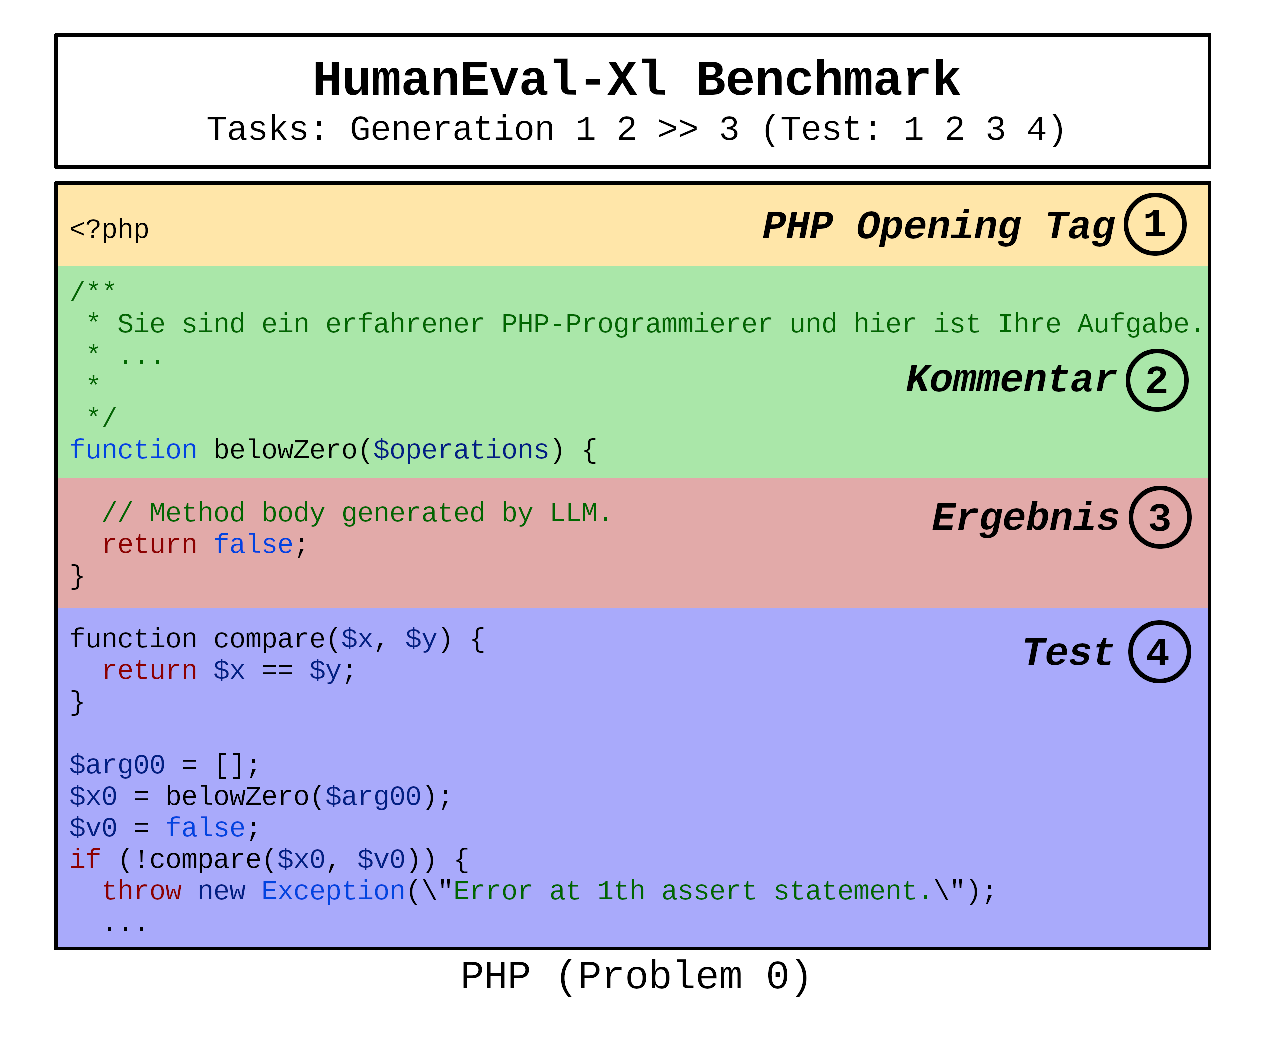
\includegraphics[width=0.6\textwidth]{content/chapter_concept_design/images/code_generation_humaneval_x.eps}
	\centering
	\caption{Aufbau des HumanEval-XL Benchmarks}
	\label{img:code_generation_humaneval}
\end{figure}

Das \textit{PHP Opening Tag}, in der Abbildung \ref{img:code_generation_humaneval} mit \textbf{1} bezeichnet, ist eine optionale Angabe zur Programmiersprache und durch den Benchmark vorgegeben. Während bei den PHP-Proben das Opening Tag \texttt{<?php} lautet, ist beispielsweise bei den JavaScript-Proben kein Opening Tag angegeben. Hier beginnt die Probe direkt mit dem Kommentar. Der in der Abbildung \ref{img:code_generation_humaneval} mit \textbf{2} bezeichnete Kommentar, enthält die eigentliche Aufgabe, die das Modell lösen soll. Auch der Kommentar ist vom Benchmark vorgegeben. Die letzte Zeile enthält den Methodennamen als Codevorgabe, der verwendet werden muss, um nach dem Generieren der Antwort abschließend einen Test durchführen zu können. Die Listings \ref{lst:example_probe_1_of_benchmark} und \ref{lst:example_probe_2_of_benchmark} zeigen Beispiele für die beiden Bereiche aus den ersten zwei Proben des Benchmarks.\vspace{0.2cm}

\begin{lstlisting}[
	language=php,
	label=lst:example_probe_1_of_benchmark,
	caption={PHP Beispiele für die erste Probe}
]
<?php

/**
* Sie sind ein erfahrener PHP-Programmierer und hier ist Ihre Aufgabe.
* Sie erhalten eine Liste von Einzahlungs- und Abhebungsvorgängen auf einem Bankkonto, das mit einem Nullsaldo beginnt. Ihre Aufgabe besteht darin, festzustellen, ob zu irgendeinem Zeitpunkt das Guthaben des Kontos unter Null fällt, und an diesem Punkt sollte die Funktion True zurückgeben. Andernfalls sollte sie False zurückgeben.
* >>> below_zero([1, 2, 3])
* False
* >>> below_zero([1, 2, -4, 5])
* True
*
*/
function belowZero($operations){
\end{lstlisting}


\begin{lstlisting}[
	language=php,
	label=lst:example_probe_2_of_benchmark,
	caption={PHP Beispiele für die zweiten Probe}
]
<?php

/**
* Sie sind ein erfahrener PHP-Programmierer und hier ist Ihre Aufgabe.
* Für eine gegebene Liste von ganzen Zahlen soll ein Tupel zurückgegeben werden, das aus der Summe und dem Produkt aller Zahlen in der Liste besteht.
* Eine leere Summe soll gleich 0 und ein leeres Produkt gleich 1 sein.
* >>> sum_product([])
* (0, 1)
* >>> sum_product([1, 2, 3, 4])
* (10, 24)
*
*/
function sumProduct($numbers){
\end{lstlisting}
	
Diese beiden Teile Opening Tag und Kommentar werden an das Modell als Eingabeaufforderung übergeben und dieses generiert den Code, welches als \textit{Ergebnis} von dem Modell zurückgeliefert wird. Das Modell sollte im Idealfall den vorgegebenen Methodennamen aufgegriffen haben und diesen für die Ausgabe des Ergebnisses verwendet. Somit findet sich der Methodenname auch im Bereich \textbf{3} wieder. Ebenfalls werden oft das Opening Tag und der Kommentar durch das Modell übernommen. In der Abbildung \ref{img:code_generation_humaneval} ist das Ergebnis mit \textbf{3} ausgezeichnet. Der Bereich \textbf{4} bildet den letzten Teil des Benchmarks. Der Test ist ebenfalls vom HumanEval-XL Benchmark vorgegeben. Hier wird ein einfacher Vergleich durchgeführt der bei Abweichung von der Vorgabe eine Exception auslöst. Dazu werden an die vordefinierte Methode Parameter übergeben, aus denen der generierte Code eine Lösung errechnet. Diese wird mit einer, durch den Benchmark vordefinierten Lösung abgeglichen. Das Listing \ref{lst:example_test_1_of_benchmark} zeigt den Aufbau des Tests, am Beispiel der ersten Probe des Benchmarks.\vspace{0.2cm}

\begin{lstlisting}[
	language=php,
	label=lst:example_test_1_of_benchmark,
	caption={PHP Beispiele für den Test der ersten Probe}
]
function compare($x, $y) {
	return $x == $y;
}
$arg00 = [];
$x0 = belowZero($arg00);
$v0 = false;
if (!compare($x0, $v0)) {
	throw new Exception("Error at 1th assert statement.");
}
$arg10 = [1, 2, -3, 1, 2, -3];
$x1 = belowZero($arg10);
$v1 = false;
if (!compare($x1, $v1)) {
	throw new Exception("Error at 2th assert statement.");
}
$arg20 = [1, 2, -4, 5, 6];
$x2 = belowZero($arg20);
$v2 = true;
if (!compare($x2, $v2)) {
	throw new Exception("Error at 3th assert statement.");
}
$arg30 = [1, -1, 2, -2, 5, -5, 4, -4];
$x3 = belowZero($arg30);
$v3 = false;
if (!compare($x3, $v3)) {
	throw new Exception("Error at 4th assert statement.");
}
$arg40 = [1, -1, 2, -2, 5, -5, 4, -5];
$x4 = belowZero($arg40);
$v4 = true;
if (!compare($x4, $v4)) {
	throw new Exception("Error at 5th assert statement.");
}
\end{lstlisting}

\subsection{Durchführung der Evaluierung}
Nach der Generierung des Codes durch das Modell werden die Bereiche \textbf{3} (Ergebnis) und \textbf{4} (Test) für die Evaluierung der Probe verwendet. Hierfür werden die Bereiche zusammengeführt und ergeben einen testbaren ausführbaren Code. Die Ergebnisse werden dokumentiert und dienen für Berechnung der Wahrscheinlichkeit, das ein Modell unter $k$-Proben eine korrekte Antwort liefert.\vspace{0.2cm}

Der Ablauf der Evaluation ist in Abbildung \ref{img:sequence_of_evaluation} dargestellt.\vspace{0.2cm}

\begin{figure}[!ht]
	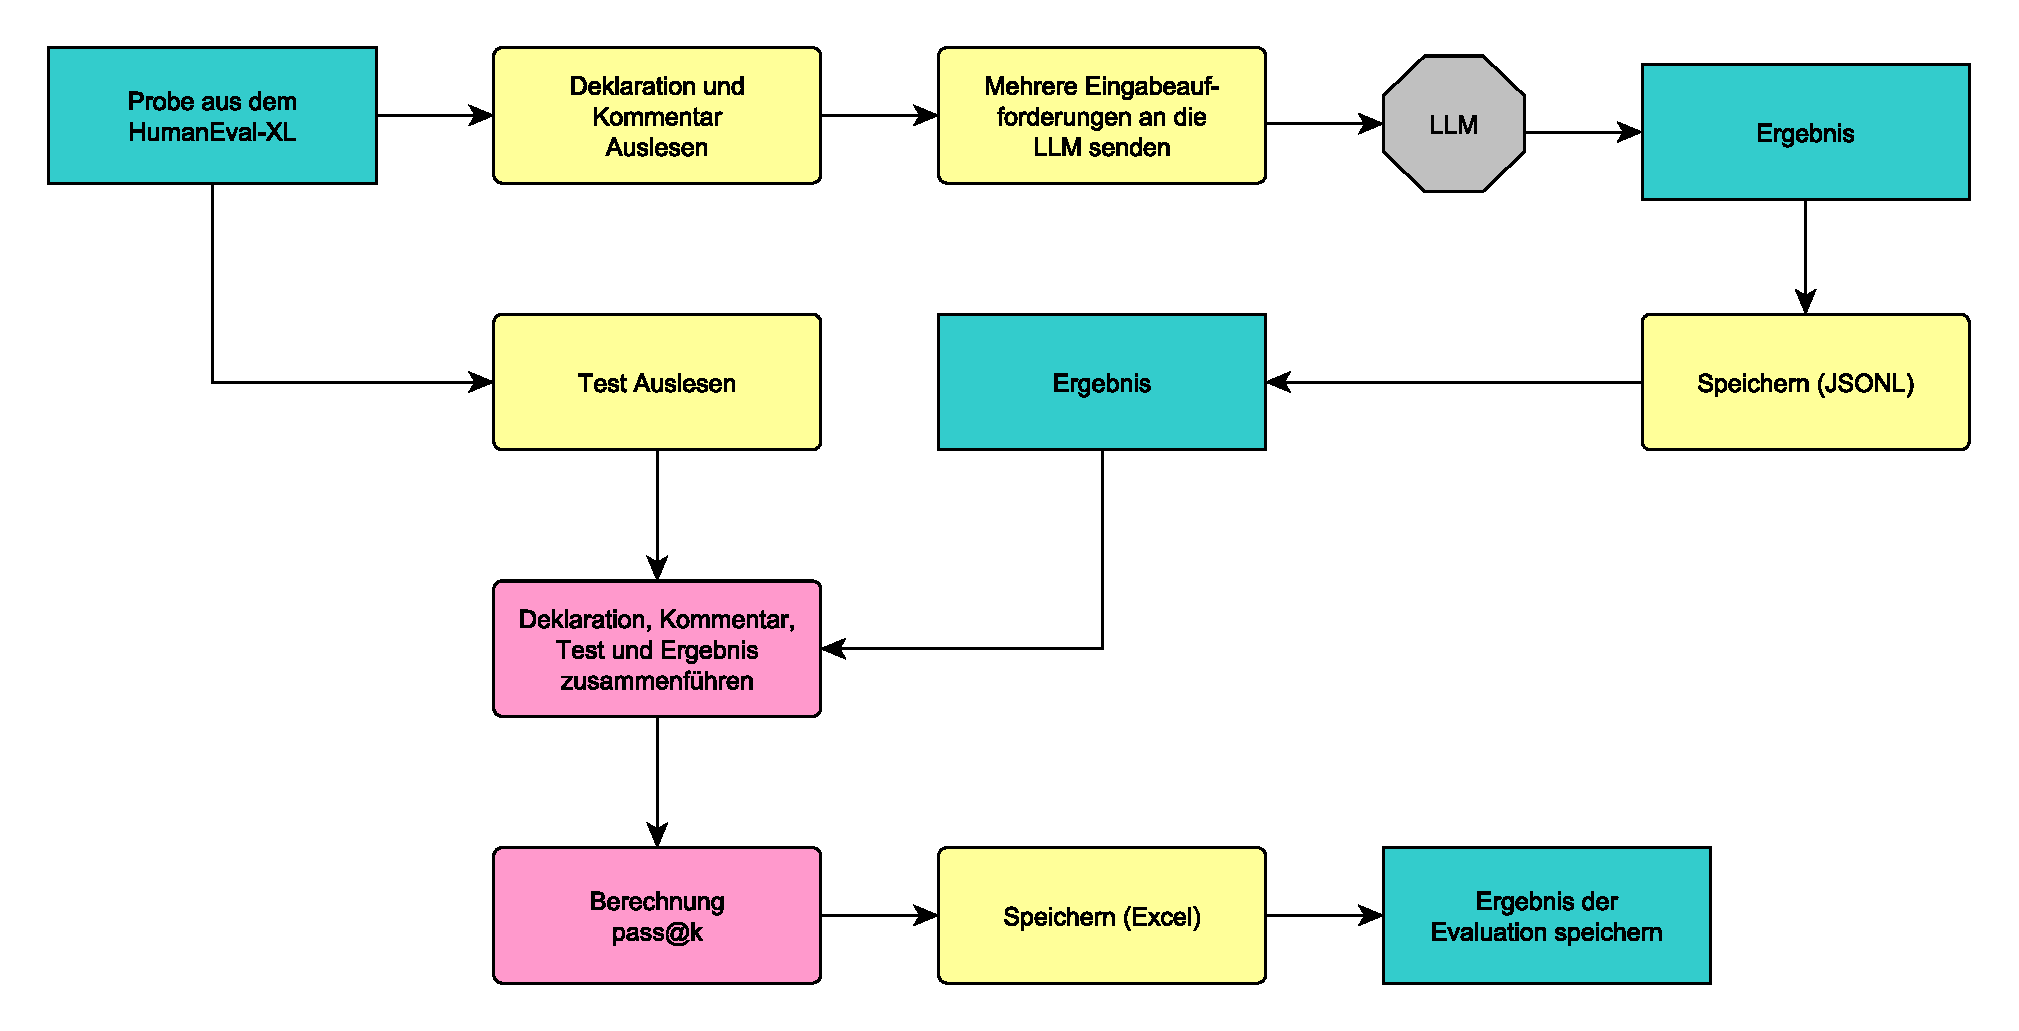
\includegraphics[width=\textwidth]{content/chapter_concept_design/images/ablauf_evaluation.eps}
	\centering
	\caption{Ablauf der Evaluierung mit dem HumanEval-XL Benchmarks}
	\label{img:sequence_of_evaluation}
\end{figure}


%*   Welche Arten von Code sollen generiert werden? (z.B. einfache HTML-Formulare, komplexe JavaScript-Funktionen, serverseitiger Code in Python/Node.js, etc.)
Um die Modelle zu evaluieren und ihre Fähigkeiten hinsichtlich der im Web vorherrschenden Programmiersprachen zu untersuchen, werden die Tests in den Programmiersprache PHP und in der deutschen Version vorgenommen. Dafür sollen die Modelle mehrfach einfache Funktionen generieren.\vspace{0.2cm}

%*   Wie werden die Testfälle für die Evaluation generiert? (z.B. manuelle Erstellung, automatische Generierung, Verwendung von bestehenden Code-Snippets, etc.) Wie groß ist der Umfang der Testfälle? (Anzahl der zu generierenden Code-Snippets)
Der Benchmark liefert jeweils einen Test für die Evaluierung mit. Dazu werden bereits in den Prompts die Namen der Methoden und die zu übergebenen Parameter angegeben, welche durch die Modelle zu erstellen sind. Der jeweilige Test verwendet dann diesen Namen und übergibt die geforderten Parameter. Das Listing \ref{lst:example_prompt_test_by_humaneval_benchmark} zeigt ein Beispiel für einen mitgelieferten HumanEval-XL Test.\vspace{0.2cm}

\begin{lstlisting}[language=php,caption={Beispiel für einen Test aus dem HumanEval-XL Benchmark},label=lst:example_prompt_test_by_humaneval_benchmark]
function compare($x, $y) {
	return $x == $y;
}
$arg00 = [3, 1, 2, 4, 5];
$x0 = median($arg00);
$v0 = 3;
if (!compare($x0, $v0)) {
	throw new Exception(\"Error at 1th assert statement.\");
}
\end{lstlisting}


%*   Wie werden die Ergebnisse der LLMs verglichen? (z.B. Vergleich mit Referenzcode, manuelle Überprüfung, automatische Tests, etc.)
Um die Modelle untereinander zu vergleichen, bekommen alle Modelle dieselben Prompts. Von jedem Prompt werden pro Modelle fünf Varianten erstellt. Die Ergebnisse werden in einer Liste chronologisch gespeichert. Mithilfe der pass@k Methode erfolgt die Evaluierung der Ergebnisse und anschließend die Bewertung der Modelle.

\subsection{Dokumentation der Daten}
Die verwendeten Dateien des Benchmarks sind im \textit{JSONL}-Format festgehalten. Ebenso werden die Ergebnisse der LLM Abfragen in diesem Format dokumentiert. Für jede Probe wurde eine separate Datei erstellt, die jeweils fünf Ergebnisse einer LLM enthält. Für den gesamten Benchmark sind pro LLM 80 \textit{JSONL}-Dateien vorhanden.\vspace{0.2cm}

Neben den Rohdaten wurden die Ergebnisse in verschiedenen \textit{Open Document Speadsheet} (ODS) übernommen. Die Dateien lassen sich mit Tabellenkalkulationstool von OpenOffice oder LibreOffice öffnen. Dies dient als Zusammenfassung der Ergebnisse und Zusätzlich wurden hieraus Grafiken generiert, welche auch in diesem Dokument Verwendung finden.\vspace{0.2cm}

Als letztes wurden die programmierten Klassen und Methoden in Python-Dateien (\texttt{*.py}) abgelegt, mit denen die Ergebnisse erstellt und evaluiert wurden. Somit lasen sich alle erhobenen Ergebnisse nachvollziehen.

%---------------------------------------------------------------------------------------------------


\section{Konzeption der Optimierung}\label{sec:conzept_of_optimization_prompt}
%*   Welche Strategien für das Prompt-Engineering werden untersucht? (z.B. Few-Shot-Prompting, Chain-of-Thought-Prompting, Verwendung von Code-Kommentaren als Prompts, etc.)
%Während die Evaluierung der Modelle ausschließlich mit den Proben des HumanEval-XL erfolgten, wird die Optimierung der Prompts, an zusätzlichen eigenen erstellten Proben erfolgen. Diese sind komplexer als die allgemeinen Proben aus dem HumanEval-XL Benchmark. Hierbei soll untersucht werden, mit welchem Ansätzen Prompts im Bereich der Codegenerierung für die Webprogrammierung erfolgen kann. Es wird neben der Proben auch ein Unittest vorgegeben. Somit kann die Codeüberprüfung der generierten Snippets mit Unittests erfolgen. Der Vorteil von Unittest ist, dass alle Tests durchgeführt werden, auch wenn ein vorheriger Test fehlschlägt. Um diese Tests ausführen zu können, sind PHP Dateien erforderlich. Somit müssen die generierten Codes in Dateien gespeichert und können im Anschluss geprüft werden.\vspace{0.2cm}

%Für die Evaluierung der Ergebnisse der Optimierung wird manuell und automatisiert erfolgen. Durch die automatisierte Evaluierung ist auch hier der Vorteil gegeben das die Ergebnisse der ausgewählten Modelle nach dem gleichen Verfahren beurteilt werden. Wie bei der Evaluierung der Modelle werden die Ergebnisse auch hier festgehalten und dokumentiert.\vspace{0.2cm}

%In der Arbeit werden verschiedene Möglichkeiten der Optimierung untersucht, die in den folgenden Kapiteln vorgestellt und deren Durchführung erläutert werden.


%\subsection{Prompt-Engineerings}
Die Prompts aus dem HunamEval-XL Benchmark sind als \textit{One-Shot-Prompts} oder \textit{Few-Shot-Prompts} verfasst. So sind neben der eigentlichen Aufgabe, noch ein oder mehrere Beispiele für die Eingabeparameter der geforderten Methode und das erwartete Ergebnis angegeben. Das Listing \ref{lst:example_prompt_by_humaneval_benchmark} zeigt ein Beispiel für einen Prompt aus dem HumanEval-XL Benchmark. Im gezeigten Beispiel wird die Aufgabe und zwei Lösungsbeispiele als Prompt an die LLM gesandt. Die Beispiele enthalten die Eingabeparameter und das geforderte Ergebnis der erwarteten Methode.\vspace{0.2cm}

\begin{lstlisting}[language=php,caption={Prompt Beispiel für  eine Aufgabe aus dem HumanEval-XL Benchmark},label=lst:example_prompt_by_humaneval_benchmark]
<?php
/**
 * Sie sind ein erfahrener PHP-Programmierer und hier ist Ihre Aufgabe.
 * Gib den Median der Elemente in der Liste l zurück.
 * >>> median([3, 1, 2, 4, 5])
 * 3
 * >>> median([-10, 4, 6, 1000, 10, 20])
 * 15.0
 */
function median($l){
\end{lstlisting}

Anders als bei \textit{Zero-Shot-Prompts}, können LLMS durch die Angabe von Beispielen die Regeln besser erlernen, Muster und Konzept der Aufgabe besser verstehen und es wird eine Verbesserung des generieren Programmcodes erreicht. Durch das Anwenden der Art von Prompts Design wurden die Eingabeaufforderungen bereits durch die Autoren des HumanEval-XL optimiert.\vspace{0.2cm}

Neben der Optimierung des Prompt Designs wurde weitere Optimierungen in den Eingabeaufforderungen des HumanEval-XL angewandt. So wurde die Eingabeaufforderung bereits als Kommentar der jeweiligen Programmiersprache verfasst. Bei der Probe für die PHP Programmierung wird vor dem Kommentar auf das, für PHP Programme erforderliche . Das definiert einen Kontextparameter und liefert für die LLM einen ersten Anhaltspunkt der zu generierenden Programmiersprache.\vspace{0.2cm}

Eine weitere Optimierung der Eingabeaufforderung ist die letzte Zeile. Hier ist bereits der Name für die erwartete Funktion angegeben. Hier wird die Fähigkeit der Modelle ausgenutzt, Funktionen und Codes zu vervollständigen. Dies ist wichtig, da die Tests im Benchmark auf einen existierenden Funktionsnamen angewiesen sind.\vspace{0.2cm}

Somit lässt sich feststellen, dass die Eingabeaufforderungen weitestgehend optimiert sind. Daher wird auf eine weitere manuelle Optimierung der Eingabeaufforderung verzichtet. Es gibt viele Arbeiten, die sich mit genau diesem Problem befassen und es sind durchaus weitere Möglichkeiten vorhanden, die Eingabeaufforderungen zu optimieren.\vspace{0.2cm}

%*   Wie werden die Prompts aufgebaut sein? (z.B. klare Anweisungen, Beispiele, Kontextinformationen, etc.)
%Bei der Optimierung der Eingabeaufforderungen werden die LLMs bei NL2Code Generierung einen objektorientierten Ansatz zu generieren. Diese generierten Klassen lassen sich mit Test-Frameworks wir \textit{phpunit} und \textit{phpmetrics} evaluieren.\vspace{0.2cm}

\subsection{Optimierung durch Frameworkauswahl}
Eine andere Methode zur Optimierung der Eingabeaufforderungen ist die Verwendung verschiedener Frameworks. Hierbei werden die Eingabeaufforderungen auf verschiedenen Arten und Weisen, je nach eingesetztem Framework angepasst und beispielsweise mit zusätzlichen Meta-Angaben versehen. Es soll untersucht werden wie sich die Verwendung unterschiedlicher Frameworks auf die Ausgaben der Modelle auswirkt. In der Arbeit werden die Auswirkungen auf die Ergebnisse der Python-Frameworks \textit{langchain} und \textit{DSPy} für verschiedene Modelle verglichen. Für einen automatisierten Test wird hier der HumanEval-XL angewandt.\vspace{0.2cm}

Das Framework \textit{langchain} wurde 2022 vorgestellt und ermöglicht Nutzern die Entwicklung komplexer Anwendungen für LLMs. Jedoch ist Fachwissen im Prompt-Engineering erforderlich, um optimale Eingabeaufforderungen an die Modelle zu stellen. Dieses Fachwissen ist beim \textit{DSPy}-Framework nicht mehr notwendig. Hier übernimmt das Framework die Optimierung der Eingabeaufforderungen für die Modelle und macht somit das manuelle optimieren der Prompts und deren Techniken überflüssig. \textit{DSPy} ist im Oktober von Forschern veröffentlicht worden die Standards für NLP arbeiten.\vspace{0.2cm}


%*   Werden verschiedene Prompt-Varianten für die gleichen Code-Generierungsaufgaben verwendet, um deren Einfluss auf die Ergebnisse zu untersuchen?
\subsection{Evaluierung der Optimierungen}
Wie auch schon bei der Evaluierung der Modelle werden die Ergebnisse festgehalten, um diese nachvollziehen zu können. Die erhobenen Rohdaten werden in Dateien, die im \textit{JSONL}-Format vorliegen gespeichert. Für die Auswertung der Ergebnisse ist auch hier das \textit{Open Document Speadsheet (ODS)} vorgesehen.\vspace{0.2cm}

Die erstellen Programme für die Erstellung der Rohdaten und der Evaluierung, sind als Python-Dateien \texttt{*.py} abgelegt, um die Nachvollziehbarkeit der Ergebnisse zu gewährleisten.
%Für die erweiterte Messung des PHP Codes kommt das Tool \texttt{phpmetrics} zum Einsatz. \texttt{phpmetrics} liefert eine Vielzahl an Metriken,mit der der Code analysiert werden kann. Bei diesem Tool liegt der Fokus auf die Ergebnisse von \texttt{Cyclomatic Complexity}, mit der die Komplexität des Codes gemessen wird. Auf den \texttt{Maintainability Index} zur Auswertung der Wartbarkeit. Diese ermittelt wie aufwändig es zukünftig ist den Code zu erweitern und bewertet die Lesbarkeit. Ein weiterer Parameter welcher hilft die Komplexität zu bewerten, ist der \texttt{Logical Lines of Code} Parameter. Ein weiteres Indiz zur Wartbar- und Lesbarkeit ist der \texttt{Method Length} Parameter. Ein weiterer Parameter zur Bewertung der Lesbarkeit ist der Parameter \texttt{Numbers of Parmeters}. Diese gibt die Anzahl der Parameter welche in die Methode übergeben werden. Eine hohe Anzahl kann ein Indiz dafür sein, das der Code schwerer zu lesen ist. Zur Bewertung der Dokumentation wird der Parameter \texttt{Comment Density} herangezogen.
%Mithilfe eines Python-Skripts wird der generierte Code mit \texttt{phpmetrics} evaluiert.\vspace{0.2cm}

%(SonarQube, wenn die Zeit es noch erlaubt)

%Mit dem SonarQube steht ein Auswertungstool zur Verfügung, welches neben qualitativen Codeanalyse noch eine Sicherheitsanalyse des Codes durchführt und die technischen Schulden ermittelt. Somit ist SonarQube eine Ergänzung zu \texttt{phpmetrics}. SonarQube wird eine lokale VM ausgeführt und mittels Integration werden die generierten Codes an den Server übermittelt.\vspace{0.2cm}

%Beide Verfahren \texttt{phpmetrics} und \texttt{SonarQube} benötigen für die Analyse Dateien. Somit müssen die Ergebnisse erst als Datei gespeichert werden, bevor die Tools mit der Analyse beginnen.


%*   Dieser Abschnitt ist besonders wichtig, da er sich mit der Optimierung der LLMs durch Prompt-Engineering beschäftigt.

%---------------------------------------------------------------------------------------------------


\section{Testumgebung}
%*   Welche Hardware und Software werden für die Experimente verwendet? (z.B. CPU, GPU, Betriebssystem, Programmiersprachen, Bibliotheken, etc.)
Die \textit{Open-Source}-Modelle laufen auf einem Debian 12 System, welches mit 8 Kernen (16 Threads) und 32 GB RAM ausgestattet ist. Um zusätzlichen Speicher zu erhalten, wurde eine 100 GB Swap Partition genutzt. Zur Unterstützung wurde eine RTX 3060 Grafikkarte der Firma Nvidia, 12 GB VRAM verbaut. Für die Bereitstelle ist das freie Framework Ollama zum Einsatz gekommen.\vspace{0.2cm}

Über die Hard- und Softwarekomponenten der kommerziellen \textit{Cloused-Source}-Modelle sind keine Hardwarespezifikationen oder andere tiefer gehende Informationen vorhanden. Da die Performance für die Evaluierung keine entscheidende Rolle spielt, wird nicht weiter und tiefer gehend recherchiert. \vspace{0.2cm}

Alle wichtigen Codes und Codesequenzen, sowie die Ergebnisse sind im Dokument oder im Anhang zu finden. Der gesamte Code und Ergebnisse sind dokumentiert, sodass die Möglichkeit besteht die Evaluierungen nachzuvollziehen. Alle Daten und Dateien werden unter \href{https://github.com/willi-pahl/master-thesis}{https://github.com/willi-pahl/master-thesis} bereitgestellt.\vspace{0.2cm}

%*   Wie wird die Reproduzierbarkeit der Experimente sichergestellt? (z.B. Verwendung von Versionskontrolle, Dokumentation der Umgebung, etc.)

